\section{Software Introduction}
This part describes the software of the Linux based components.
The FPGA software is described elsewhere in detail, but the
interfaces are described here, as well as the data formats.
\begin{compactitem}[$\diamond$]
\item Functional components
\item Data streams
\item Communication and control
\item User interfaces
\end{compactitem}

\section{Data streams overview}
\begin{figure}[htb]
\centering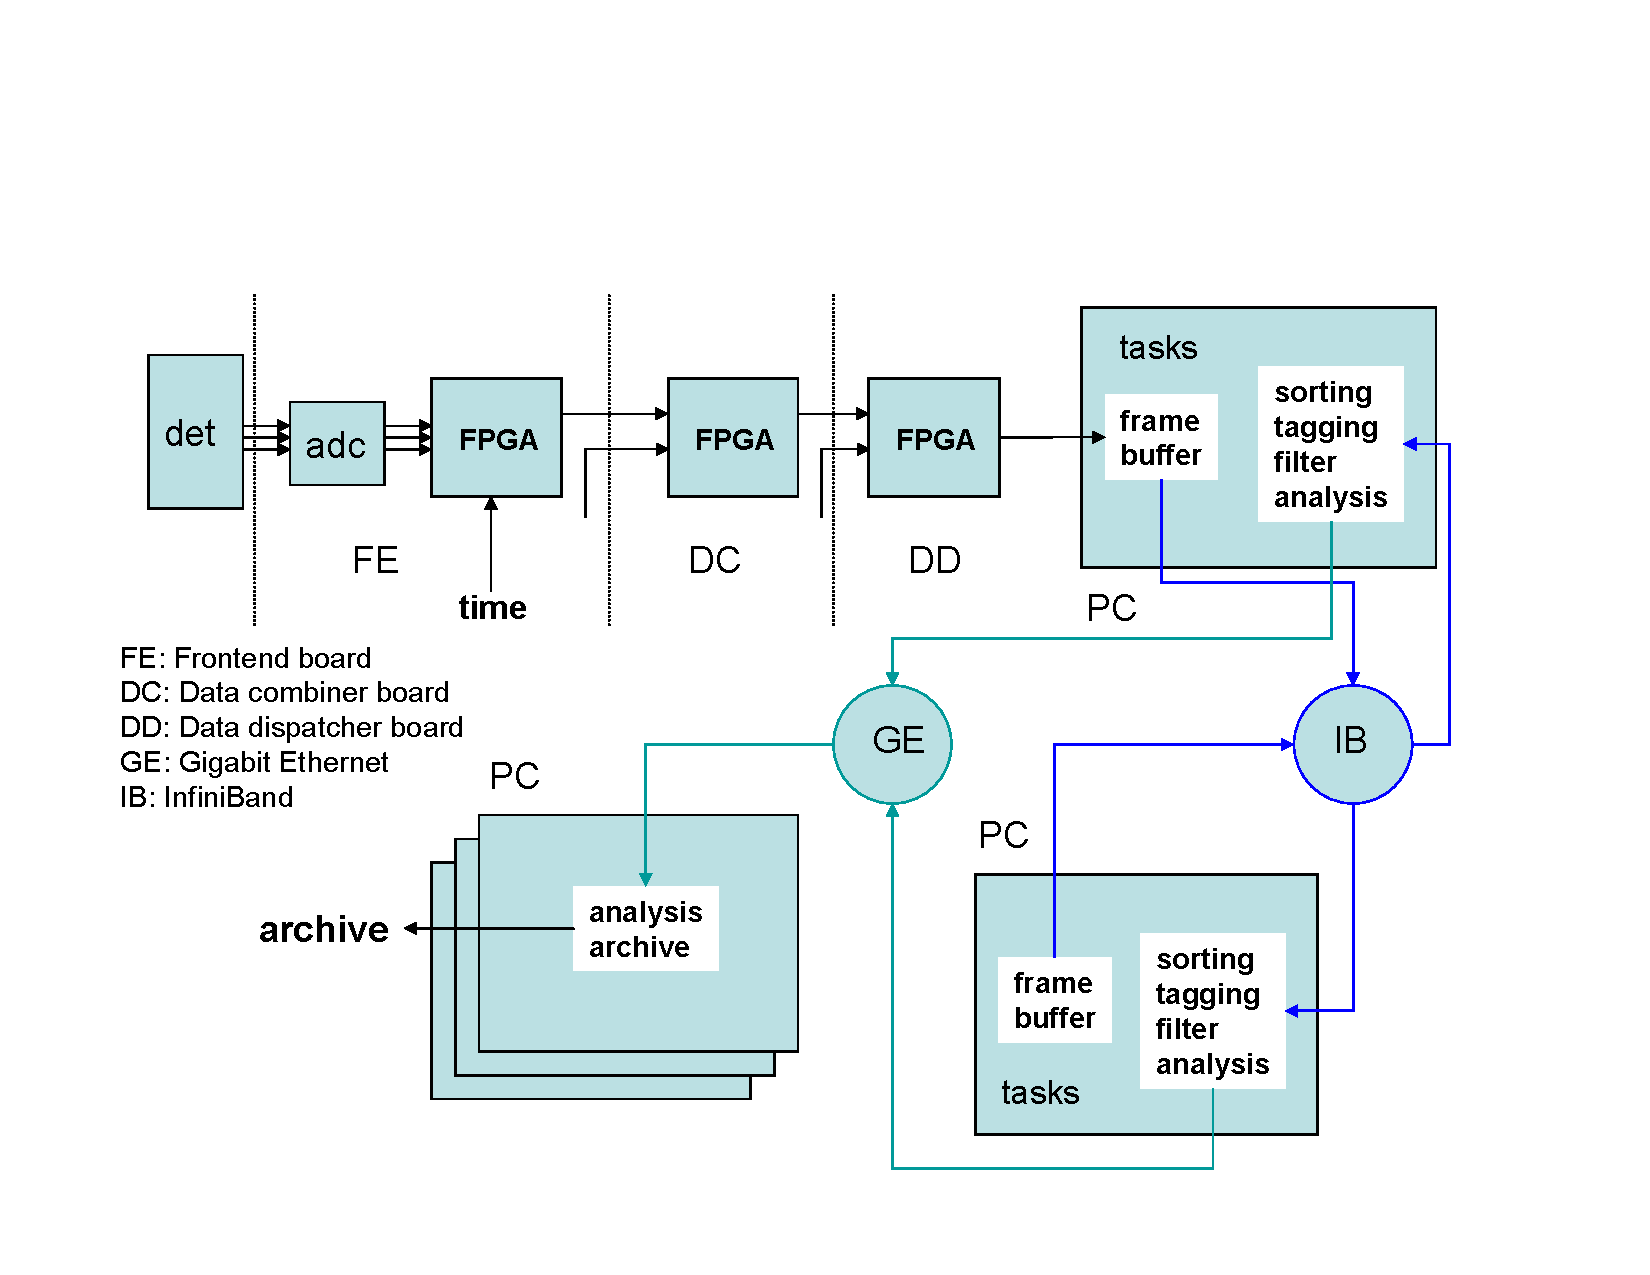
\includegraphics[width=.8\textwidth]{sw-over} % pdf file
\caption{Overall data streams architecture}
\label{fig:SW-over} % give it a name for references
\end{figure}

Fig.~\ref{fig:SW-over} shows the data streams. On the FEE board the data from
the ADCs are tagged with time stamps. The data following a time stamp may be
a stream of ADC values. Certain time stamps are time epoch markers.
Data items sent by the FEE need not to be time ordered, but {\bf all items of one epoch
should be in between the epoch markers} defining an {\sl epoch buffer}.\\
Similarly, the DCB merges all incoming epoch buffers into one output stream where
all epoch buffers are subsequent.
The ABB collects the epoch data from the inputs (one or two) and stores them in the
frame buffer in the PC.\\
The frame buffer now contains complete streams of epoch buffers containing data
items without time order. These epoch streams can be used as switching unit.
{\bf It is assumed that all items of an epoch buffer belong to that buffer!}
Through the switching all epoch streams of one epoch are combined on one PC.
Now the data items must be reconfigured, i.e. time sorted and eventually reformatted.
By multiplicity histograms over time the event time intervals can be calculated.
The data items inside this interval build the event which is tagged.

\section{Data formats}
All FEE run asynchronously. Let use term \"hit\" (whatever it means) as minimum portion of
data, which is provided by detector. Hit data size (excluding
detector channel id and time stamp) will be about 1-8 bytes depending of detector system.
Each hit should be assigned with the time stamp. Most probably, not individual hits but
rather group of hits will be assigned with the same time stamp. Required resolution
for time stamp depends on detector type. For most detectors 1 ns will be enough, for
other 50 ps is required.

\subsection{Proposal for data format}
\hyperdef{sw}{data}{[Marker: sw.data]}\\
Lets introduce following types for markers:

\begin{table}[h]
\centering
\begin{tabular}{|p{1.0cm}|p{2.0cm}|p{1.0cm}|p{10.0cm}|} \hline

Value & Name &   Marker & description \\ \hline
0000  &  Epoch & M &
Value of time epoch in 10 $\mu$s units. 28 bits can provide unique code for each
epoch inside \~ 2500 s time interval. \\ \hline
0001  &  time shift & T &
To achieve 1 ns precision of time shift inside 10 $\mu$s epoch, 13-14 bits are required.
For the 25 ps precision 19 bits can be used.
Probably, one should use rest 9 bits as size indicator how many data assigned to this time marker.
This allows fast navigation in packet to find given time value, which is important in time sorting
algorithm. \\ \hline
0010  &  channel identifier & ID &
About 10 Mchannels are expected [1] (excluding MAPS). 28-bits code can be divided on
two-three groups to have: clear system number like STS, TRD etc, subsystem number STS1,
TRD2 etc, channel inside subsystem. Should exists clear algorithm to define size of data
for given channel id (something like lookup table). \\ \hline
0011  &  Event tag & TG &
28 bits allows \~ 2.5 108 codes for events or about 25 sec for repetition of the same
code at 107 events/sec rate. \\ \hline
0100   & Histogram & H1 &
28 bits can include initial time shift and size of histogram. \\ \hline
0101  &  Peak & P &
28 bits is used for time shift (\~ 13 bits), amplitude (9 bits), width (6 bits) \\ \hline
0110   & Schedule & SCH &
28 bits used to specify schedule size. Schedule include dependency between time,
event tag and event builder, which should receive event data. \\ \hline
\end{tabular}
\caption{List of data types.}
\label{SW-data-format}
\end{table}

One can imagine a lot of variants to code data to the binary arrays.
Probably, one can formulate some rules, which allows more clearly define format. For instance:
\begin{compactitem}[$\bullet$]
\item all data flows can be separated by packet of variable size;
\item should exists simple algorithm to merge data of several packets into one;
\item data of following packet should not depend from previous one;
\item all entities of the system should use same format.
\end{compactitem}
Probably, there are other rules, which can be specified.
Lets try to define format, which conform to this rule. For instance:
\begin{compactitem}[$\bullet$]
\item any data inside package are represented as array of 4 bytes values;
\item some of this four-bytes values are defined as markers;
\item marker include 4-bit type and 28-bit data parts;
\item any packet should be started from such marker value;
\item should exists clear algorithm to navigate from marker to marker inside packet;
\item data between markers is of any kind binary data, rounded to 4 bytes.
\end{compactitem}

This list (\ref{SW-data-format} can be further extended to have unique identifier for any markers in all packets,
used in the system. It is supposed, that address information and packet length are provided
by transport protocol.\\
Data packet, coming from FEE, can be:
\begin{verbatim}
M   1        epoch marker
T   17       time shift inside epoch
ID  15       detector channel id, where hit is detected
   100  200  detector specific data
T   68       time shift of next hit
ID  34       detector channel id for next hit
    20
T  134
ID  18       this detector may not require any data
T  135
ID  19
   100  200
\end{verbatim}
